
%%%%%%%%%%%%%%%%%%%%%%%%%%%%%%%%%%%%%%%%%
% Beamer Presentation
% LaTeX Template
% Version 1.0 (10/11/12)
%
% This template has been downloaded from:
% http://www.LaTeXTemplates.com
%
% License:
% CC BY-NC-SA 3.0 (http://creativecommons.org/licenses/by-nc-sa/3.0/)
%
%%%%%%%%%%%%%%%%%%%%%%%%%%%%%%%%%%%%%%%%%

%----------------------------------------------------------------------------------------
%	PACKAGES AND THEMES
%----------------------------------------------------------------------------------------

\documentclass{beamer}

\mode<presentation> {

% The Beamer class comes with a number of default slide themes
% which change the colors and layouts of slides. Below this is a list
% of all the themes, uncomment each in turn to see what they look like.

%\usetheme{default}
%\usetheme{AnnArbor}
%\usetheme{Antibes}
%\usetheme{Bergen}
%\usetheme{Berkeley}
%\usetheme{Berlin}
%\usetheme{Boadilla}
%\usetheme{CambridgeUS}
%\usetheme{Copenhagen}
%\usetheme{Darmstadt}
%\usetheme{Dresden}
%\usetheme{Frankfurt}
%\usetheme{Goettingen}
%\usetheme{Hannover}
%\usetheme{Ilmenau}
%\usetheme{JuanLesPins}
%\usetheme{Luebeck}
\usetheme{Madrid}
%\usetheme{Malmoe}
%\usetheme{Marburg}
%\usetheme{Montpellier}
%\usetheme{PaloAlto}
%\usetheme{Pittsburgh}
%\usetheme{Rochester}
%\usetheme{Singapore}
%\usetheme{Szeged}
%\usetheme{Warsaw}

% As well as themes, the Beamer class has a number of color themes
% for any slide theme. Uncomment each of these in turn to see how it
% changes the colors of your current slide theme.

%\usecolortheme{albatross}
%\usecolortheme{beaver}
%\usecolortheme{beetle}
%\usecolortheme{crane}
%\usecolortheme{dolphin}
%\usecolortheme{dove}
%\usecolortheme{fly}
%\usecolortheme{lily}
%\usecolortheme{orchid}
%\usecolortheme{rose}
%\usecolortheme{seagull}
%\usecolortheme{seahorse}
%\usecolortheme{whale}
%\usecolortheme{wolverine}

%\setbeamertemplate{footline} % To remove the footer line in all slides uncomment this line
%\setbeamertemplate{footline}[page number] % To replace the footer line in all slides with a simple slide count uncomment this line

%\setbeamertemplate{navigation symbols}{} % To remove the navigation symbols from the bottom of all slides uncomment this line
}
\usepackage[ampersand]{easylist}
\usepackage{graphicx} % Allows including images
\usepackage{booktabs} % Allows the use of \toprule, \midrule and \bottomrule in tables

%----------------------------------------------------------------------------------------
%	TITLE PAGE
%----------------------------------------------------------------------------------------

\title[Unbounded Orchestrations for Manufacturing]{Unbounded Orchestrations of Transducers for Manufacturing } % The short title appears at the bottom of every slide, the full title is only on the title page

%\author[E{E.~Puglisi \and M.~Persiani \and F.~Frattolillo}
\author[E.Puglisi,M.Persiani,F.Frattolillo]{Natasha Alechina, Tom\'{a}\^{s} Br\'{a}zdil, Giuseppe De Giacomo, Paolo Felli, Brian Logan, Moshe Y. Vardi} % Your name 
\institute[Sapienza] % Your institution as it will appear on the bottom of every slide, may be shorthand to save space
{
Presented by E.Puglisi,M.Persiani,F.Frattolillo \\
Sapienza University \\ % Your institution for the title page
%\medskip
%\textit{john@smith.com} % Your email address
}
\date{May 17,2019} % Date, can be changed to a custom date

\begin{document}

\begin{frame}
\titlepage % Print the title page as the first slide
\end{frame}

\begin{frame}
\frametitle{Overview} % Table of contents slide, comment this block out to remove it
\tableofcontents % Throughout your presentation, if you choose to use \section{} and \subsection{} commands, these will automatically be printed on this slide as an overview of your presentation
\end{frame}

%----------------------------------------------------------------------------------------
%	PRESENTATION SLIDES
%----------------------------------------------------------------------------------------

%------------------------------------------------
\section{Introduction} % Sections can be created in order to organize your presentation into discrete blocks, all sections and subsections are automatically printed in the table of contents as an overview of the talk
%------------------------------------------------


%\subsection{Subsection Example} % A subsection can be created just before a set of slides with a common theme to further break down your presentation into chunks

% PAGE3
\begin{frame}[fragile]
\frametitle{Introduction}
\begin{easylist}[itemize]
& Let's give some definitions:
&& \textbf{process plan:} specifies the specific \textit{manufacturing resources} to be used for each manufacturing and assembly operations, and how materials and parts move between the various manufacturing resources 
&& \textbf{manufacturing resources:} computer, robots etc.
&& \textbf{process recipe:} set of abstract manufacturing tasks.
& Reasons behind this study:
&& Process planning is traditionally carried out by manufacturing engineers and is largely a manual process.
&& Such process is uneconomic for the small batch sizes typical of the manufacturing as a service model.
&& There is an increasing interest in using synthesis to automate the synthesis of manufacturing process planning
\end{easylist}
\end{frame}

%PAGE4
\begin{frame}[fragile]
\frametitle{Introduction}
\begin{easylist}[itemize]
& Sometimes the products to be manufactured are not known in advance and are often produced in small batches to tight timescales. 
& We consider the problem of whether a product can be manufactured given sufficient resources.
& Only the types of available manufacturing resources are given, and we want to know whether is possible to manufature a product using only resources of those types, and, if so, how many resources of each type are needed.
\end{easylist}


\end{frame}

%------------------------------------------------
\section{Uni-Transducer}
%------------------------------------------------
%PAGE5
\begin{frame}
\frametitle{Uni-Transducers}
A \textbf{Transducer} is a finite deterministic automaton with outputs.\\ A Uni-transducer take a single input and produce a single output in each state. \\
We consider tranducer which are \textit{Mealy machine}.

\begin{block}{Uni-Transducer}
A (uni-)transducer $T = (\Sigma, \Delta, S, s_{0}, f, g)$ is a deterministic transition system with inputs and outputs, where $\Sigma$ is the \textit{input alphabet}, $\Delta$ is the \textit{output alphabet}, S is the \textit{set of states}, $s_{0}$ is the \textit{initial state}, $f: S x \Sigma \mapsto S$  is the \textit{transition function} and $g: S x \Sigma \mapsto \Delta$ is the \textit{output function}.

\end{block}
We will consider both manufacturing resources and process recipes as uni-transducers.

\end{frame}

%------------------------------------------------
\section{Orchestration Problem}
%------------------------------------------------
%PAGE6
\begin{frame}[fragile]
\frametitle{Orchestration Problem}
\begin{easylist}[itemize]
& We have a set of \textit{available transducer types} $\{T_{0},...,T_{m}\}$
& Where $T_{j} =(\Sigma, \Delta, S{j}, s_{0j}, f_{j}, g_{j}) $ represents a manufacturing resource and all $T_{j}$'s are over the same input and output alphabet.
& T represents a \textit{process recipe} which is a transducer with the same input and output as the $T_{j}$'s.
\end{easylist}

\begin{block}{Unbounded Orchestration}
The unbounded orchestration problem is to combine some numbers $n_{j}$ of resources of each type $T_{j}$ to be able to mach the \textit{behavior} of T.

\end{block}

\end{frame}

%------------------------------------------------
%PAGE7
\begin{frame}
\frametitle{Orchestration Problem}
\begin{block}{Behaviour of T}
The behaviour of T on input $\omega = a^{0},a^{1},...$ is described by the following sequence of states and outputs:\\
$T^{s}(a^{0})=f(s_{0},a^{0})$\\
$T^{o}(a^{0})=g(s_{0},a^{0})$\\
...\\
$T^{s}(a^{0},...,a^{i})=f(T^{s}(a^{0},...,a^{i-1}),a^{i})$\\
$T^{o}(a^{0},...,a^{i})=g(T^{s}(a^{0},...,a^{i-1}),a^{i})$\\
The observable output sequence of T on input $\omega$ is:\\
$ \tau^{o}_{\omega,T}= T^{o}(a^{0}),...,T^{o}(a^{0},...,a^{i})... $

\end{block}

\end{frame}

%PAGE8
\begin{frame}
\frametitle{Orchestration Problem}
\begin{block}{Controller}
Consider the transducer corresponding to the whole production facility:\\$P = T_{1,1} x...x T_{1,n_{1}} x ... x T_{m,1}x... x T_{m,n_{m}}$\\ 
where $n_{j}$ is the number of copies of every transducer type $T_{j}$.\\
A \textit{controller} for P is a function \\
$C : \Sigma^{+} \mapsto \{(1,1),...,(m,n_{m})\}$ \\
That, for each finite input string, picks a transducer in P to make a transition. The sequence of states generated by the controller on inputs $\omega$ is: \\
$\tau^{s}_{\omega,T}=(S^{0}_{1,1},...,S^{0}_{m,n_{j}}),...,(S^{i}_{1,1},...,S^{i}_{m,n_{j}}),...$\\
where only one of the local state changes in each transition:\\
$s_{h}^{i+1} = f_{h}(s^{i}_{h},a^{i}) \qquad if\quad C(a^{0},...,a^{i}) = h $\\
$s_{h}^{i+1} = s_{h}^{i} \qquad \qquad  if \quad C(a^{0},...,a^{i})\neq h$
\end{block}
\textbf{orchestration problem}: check if there are numbers of copies of each transducer type such that there is a controller C for P which realizes T.
\end{frame}



%------------------------------------------------
\section{Multi-Dimensional energy game}
%------------------------------------------------
%PAGE9
\begin{frame}
\frametitle{Multi-Dimensional energy game}
The unbounded orchestration problem can be reduced to a decidable problem on \textit{multi-dimensional energy games}.
\begin{block}{multi-dimensional energy game}
A multi-dimensional energy game is a tuple $G=(Q,R)$\\
\textbf{Q:} is a finite set of states\\
\textbf{R:} is a finite set of transitions of the form $(q_{1},op,q_{2})$\\
\textbf{C:} finite set of counters.\\
\textbf{op:} $\{0,-1,1\}^{n}$ is an update vector for the value of the counters.\\
\textbf{counter evalutation:} $\nu : C \mapsto Z$ maps every counter to a set of integers.
\textbf{configuration:} $\gamma$ is a pair (q,$\nu$), where $q\in Q$ \\
\textbf{transition:}  between two configuration $\gamma_{1} \mapsto^{t} \gamma_{2}$ ($t\in R$)is valid if $\nu_{2}= \nu_{1}+op$.\\
\textbf{history: } is a finite sequence of configurations\\
\textbf{strategy:} for a Player $i\in\{0,1\}$ is a function $\sigma_{i}$
that assigns to each history ending in a configuration $\gamma$ a possible transition.
\end{block}

\end{frame}

%------------------------------------------------
%PAGE10
\begin{frame}
\frametitle{Multi-Dimensional energy game}
\begin{block}{Winning strategy}
Player 0 \textbf{wins the game} in $\gamma$ if it wins every play starting on $\gamma$.\\
\textbf{Winning game:} a configuration for a player  is winning if $v_{k}(c) \ge 0$ for all $k \ge 1 $ and $c \in C$.\\
\textbf{Winning set:} the set $W(G,0)$ is the set of configurations $\gamma$ in which the player 0 wins. \\
\textbf{Pareto frontier:} is \textit{min}$(W(G,0))$.\\
The Pareto frontier is computable in \textbf{doubly exponential time} and 
\textbf{pseudo-polynomial} assuming the number of counters is fixed. The maximum norm of the Pareto frontier are bounded by an exponential value in the number of counter \textit{n} and polynomial in the number of states and transitions. 

\end{block}

\end{frame}

\begin{frame}
\frametitle{Pareto Frontier}
\begin{block}{Pareto Efficiency}
State of allocation of resources in which it's impossible to re-allocate so to improve any individual evaluation criterion without worsening at least another one. (i.e. an optimal configuration)
\end{block}
\begin{block}{Pareto Frontier}
The set of all the \textit{pareto efficient} allocations for a given set of resources.
\end{block}
In our case the resources to allocate are the transducer type counters stored in vector $\nu$.
\end{frame}


%------------------------------------------------
\section{Orchestrator Synthesis}
%------------------------------------------------

\begin{frame}
\frametitle{Orchestrator Synthesis}
Let's see how to reduce the \textbf{orchestration problem to a multi-dimensional energy game}. 
\newline
\newline
We are given \textit{m} resource transducer types:\\
 $T_{i}=(\Sigma,\Delta,P_{i},p_{0}^{i},\alpha _{i},\beta _{i})$\\
and a target process recipe:\\
$T =(\Sigma,\Delta,S,s_{0},f,g)$\\
The realizability problem for $\prod T_{i}^{n_{i}}=T_{1,1}x...xT_{1,n_{1}}x...xT_{m,1}x...xT_{m,n_{m}}$ can be formulated as a game between Controller(player 0) and Adversary(player 1).
The game starts with adversary choosing a symbol from the input alphabet $\Sigma$ and the controller must choose a component $T_{i,j}$ where $i \in \{ 1,...,m \}$ and $j\in \{ 1,...,n \} $. \\
Controller must be able to keep playing forever without causing a mismatch of outputs between T and $\prod T_{i}^{n_{i}}$.

\end{frame}


\begin{frame}
\frametitle{Orchestrator Synthesis}
We can describe $\prod T_{i}^{n_{i}}$ as an integer vector\\
$v=(v_{0}^{1},...,v_{k_{1}-1}^{1},...,v_{0}^{m},...,v_{k_{5}-1}^{m})$\\
where $k_{i}$ is the cardinality of the set of states of $T_{i}$ and $v_{0}^{i}+...+v_{k_{i}-1}^{i}=n_{i}$\\
Where $v^{i}_{q}$ represents the number of copies of $T_{i}$ in the state $p_{q}^{i}$\\
The game starts with all the copies of all the transducers in the state $s_{0}$, hence for each transducer $T_{i}$ the corresponding vector $v_{i} $ is $(n_{i},0)_{i}$  \newline \newline
The vector v representing the counter evaluation is updated by adding the update vector $u=(u_{0},...,u_{k_{m}-1}^{m})$ where $u_{q}^{i} = -1$ and $u_{q}^{i} = 1$ and all other components are 0. This operation represents the transition between two states of one of the available resource transducers.

\end{frame}

%PAGE25
\begin{frame}[fragile]
\frametitle{Orchestrator Synthesis}
Now we can define the following multi-dimensional energy game $G_{T_{1},...,T_{m},T}$:
\begin{easylist}
& The state set of $G_{T_{1},...,T_{m},T}$ is $(S x \Sigma )\cup S$ where 
$(S x \Sigma )$ represent all the combination of input symbol and states of T (including the error states). $Q_{0} = (S x \Sigma ) $ are the states of player 0 and $Q_{1} = S$ are the states of player 1.
& For each transition $(s,a,b,t)$(initial state, input symbol, output, new state) of T, we have in $G_{T_{1},...,T_{m},T}$ the transition $((s,a),u,t)$ for all  $u \in U_{a,b}$ (player 0's moves) and a transition $(s,0,(s,a))$ (player 1's moves).

\end{easylist}
\end{frame}



%------------------------------------------------
\section{Example}
%------------------------------------------------
%PAGE17
\begin{frame}
\frametitle{Example}
\begin{figure}
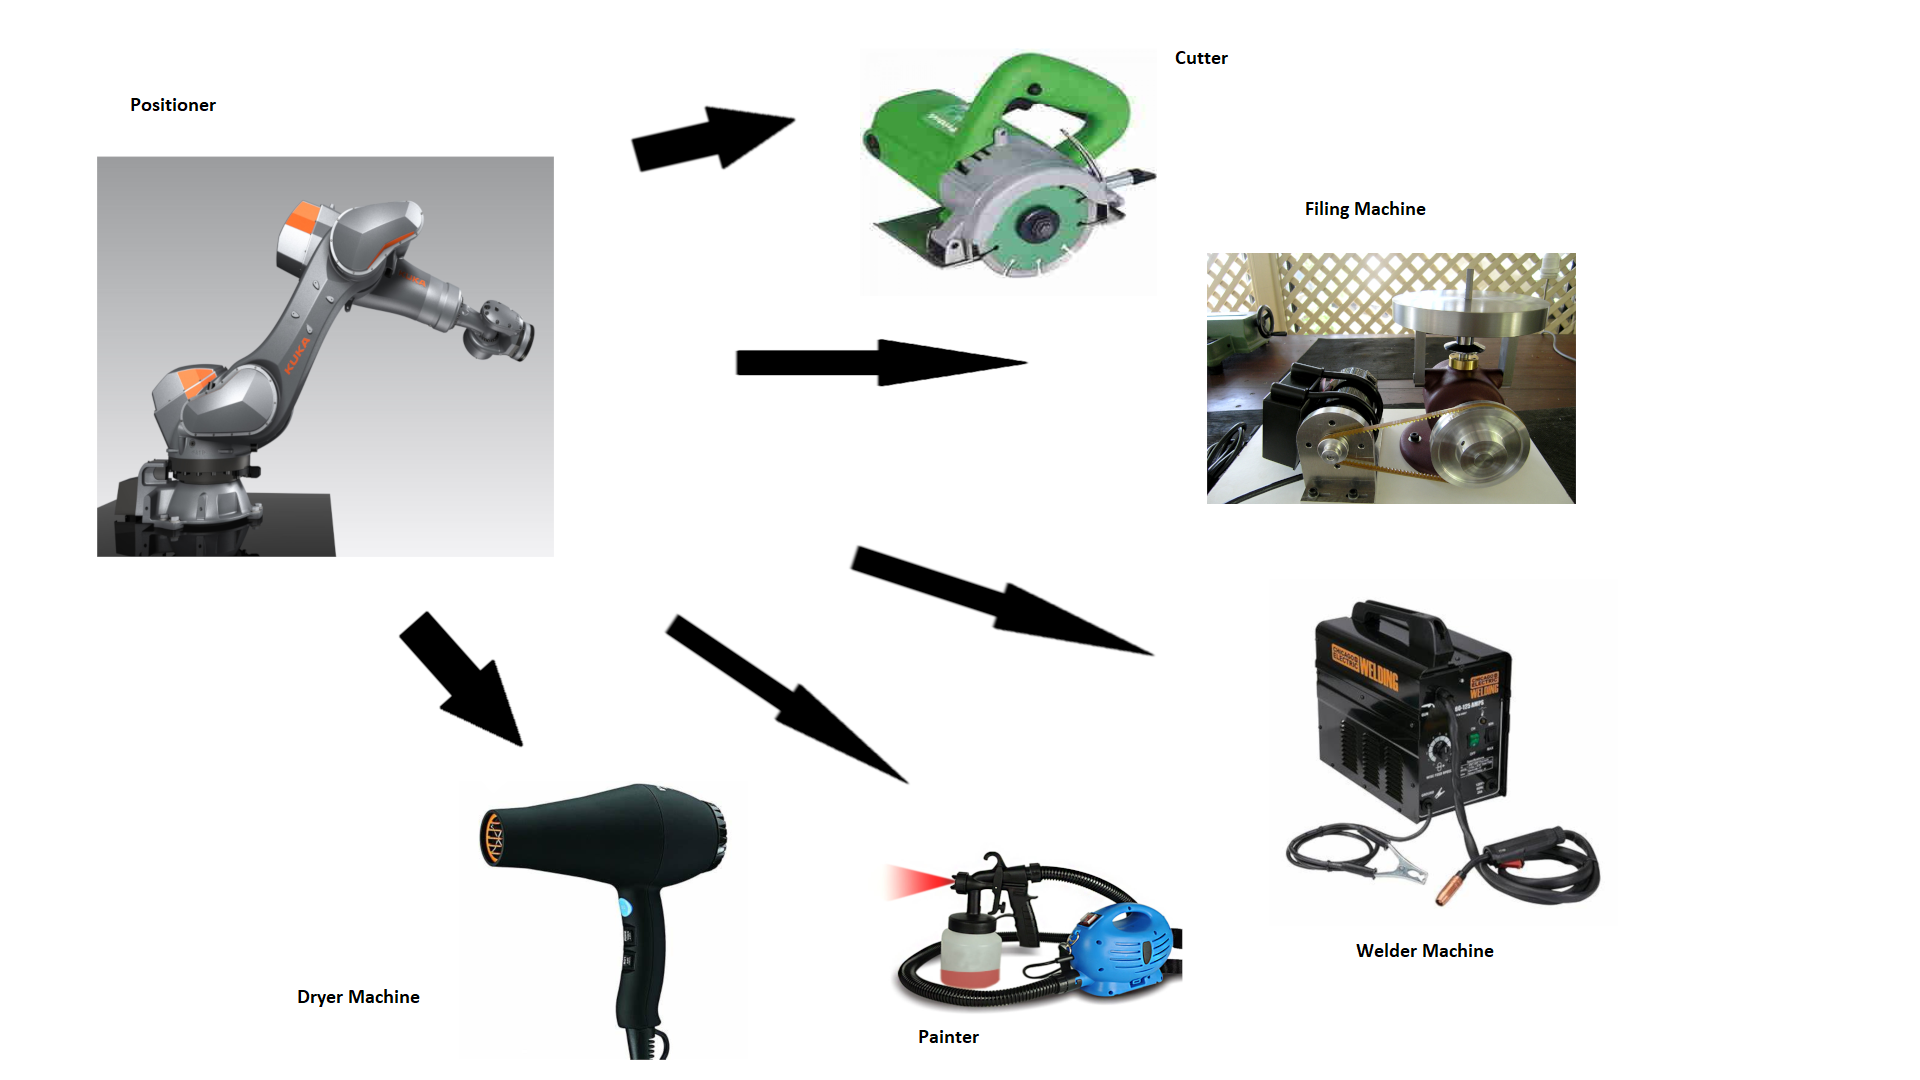
\includegraphics[width=0.8\linewidth]{process}
\end{figure}

\end{frame}

%PAGE18
\begin{frame}[fragile]
\frametitle{Example}
\begin{easylist}[itemize]
Given two metal objects, the manufacturing recipe require to: 
& Position both the objects on the \textbf{cutting machine} and cut them.
& Position the objects on the \textbf{Filing machine} and file them. 
& Position the objects on the \textbf{Welder machine} and weld them.
& Position the objects on the \textbf{Paint machine} and both paint  and dry it.
& Release the object. 
\end{easylist}

\end{frame}

%PAGE19
\begin{frame}
\frametitle{Example}
\begin{figure}
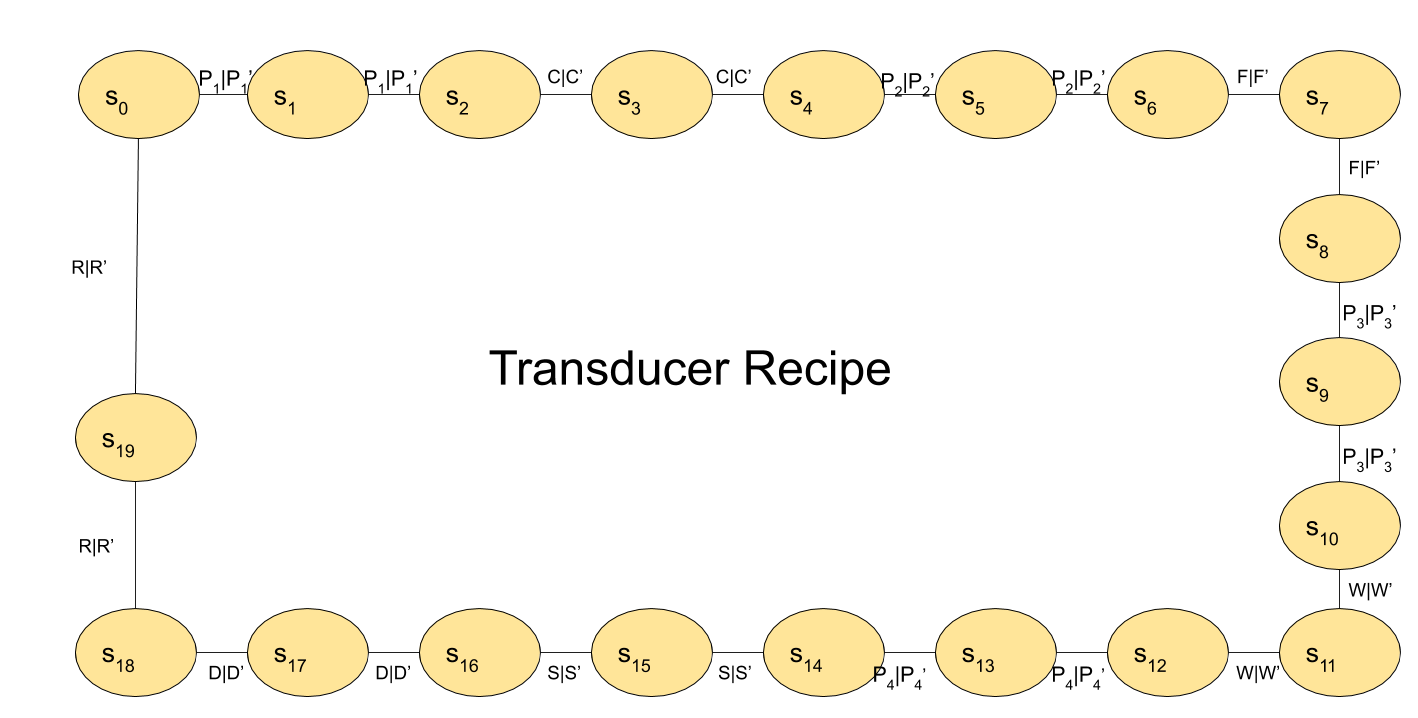
\includegraphics[width=0.8\linewidth]{ProcessRecipe}
\end{figure}

\end{frame}

%PAGE20
\begin{frame}
\frametitle{Example}
\begin{figure}
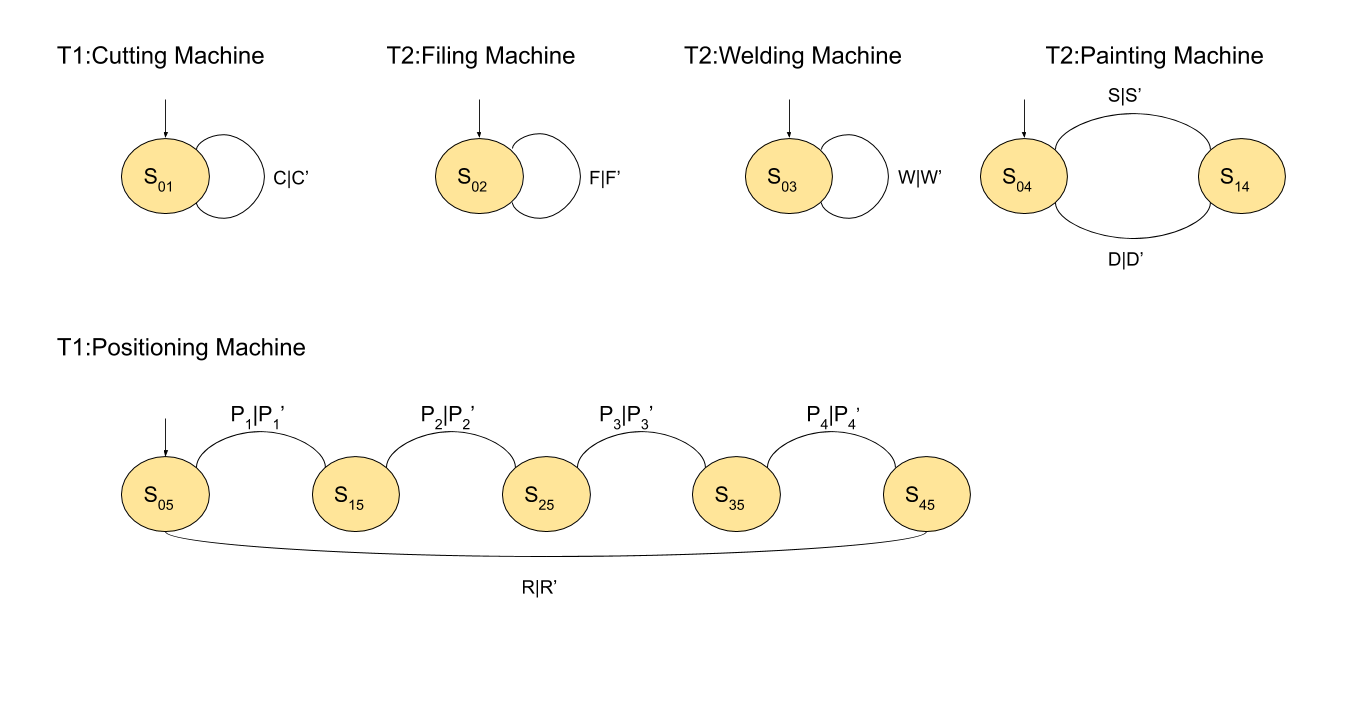
\includegraphics[width=0.9\linewidth]{ManufacturingResources}
\end{figure}
\end{frame}


%PAGE21
\begin{frame}[fragile]
\frametitle{Example}
\begin{easylist}
Our process recipe is defined as a quintuple $T=(\Sigma,\Delta,S,s_{0},f,g)$ where:
& $\Sigma = \{P_{1},P_{2},P_{3},P_{4}, C, F, S, D, R, W\}$
& $\Delta = \{P_{1}',P_{2}',P_{3}',P_{4}', C', F', S', D', R', W'\}$
& $S = \{s_{0},s_{1},...,s_{19},s_{err} \} $
& $f = \{ f(s_{0},P_{1})=s_{1},...,f(s_{19},R)=s_{0} \} $
& $g = \{ g(s_{0},P_{1})=P_{1}',...,g(s_{19},R)=R' \}$
\end{easylist}
Let's define the transducer corresponding to the whole production facility as:\\ 
$P = \prod_{i}^{n_{i}} T_{i}= T_{1,1}x...xT_{1,n_{1}}x...xT_{5,1}x...xT_{5,n_{5}}$\\
where $n_{j}$ is the number of copies of the transducer $T_{j}$.
\end{frame}

%PAGE22
\begin{frame}[fragile]
\frametitle{Example}
Our controller will be a function $C: \Sigma^{+} \mapsto \{ (1,n_{1}),...,(5,n_{5}) \}$\\
Now let's reformulate our problem as a multi-dimensional energy game.
We are given: \\ 
\begin{easylist}
& 5 resource transducers \textbf{types} $T_{i} = (\Sigma,\Delta,P_{i},p_{0}^{i},\alpha_{i},\beta_{i}) $
& The process recipe as defined above.
& P = the transducer corresponding to the whole production facility. 
\end{easylist}
This game is played by two player:
\begin{easylist}
& \textbf{Player 0:} is the Controller.
& \textbf{Player 1:} is the Adversary.
\end{easylist}
\end{frame}



%PAGE23
\begin{frame}
\frametitle{Example}
We can describe $\prod_{i}^{n_{i}}T$ as an integer vector\\
$v=(v_{0}^{1},...,v_{k_{1}-1}^{1},...,v_{0}^{5},...,v_{k_{5}-1}^{5})$\\
where $k_{i}$ is the cardinality of the set of states of $T_{i}$ and $v_{0}^{i}+...+v_{k_{i}-1}^{i}=n_{i}$\\
Where $v^{i}_{q}$ represents the number of copies of $T_{i}$ in the state $p_{q}^{i}$\\
The game starts with all the copies of all the transducers in the state $s_{0}$, hence for each transducer $T_{i}$ the corresponding vector $v_{i} $ is $(n_{i},0)_{i}$  \\

\end{frame}



%PAGE24
\begin{frame}[fragile]
\frametitle{Example}
\begin{easylist}
& The game starts with adversary choosing an input symbol $a\in \Sigma$ yielding output g(p,a) and changing the state of T to f(s,a).
& The controller must choose a copy of $T_{i}$ in some state $p_{q}^{i}$ and replacing it by a copy in state $p_{r}^{i}=\alpha _{i}(p_{q}^{i},a)$. The output corresponding to this transition is $ b=\beta _{i}(p_{q}^{i},a)$.
& The previous transition is denoted by $(p_{q}^{i},a,b,p_{r}^{i})$
& The vector v representing the counter evaluation is updated by adding the \textit{update vector u} $=(u_{0},...,u_{k_{m}-1}^{m})$ where $u_{q}^{i}=-1$ and $u_{q}^{i}=1$ and all other components are 0. $U_{a,b}$ is the set of such update vectors for transition with input $a \in \Sigma$ and output $b \in \Delta$.

& Controller must be able to play forever without causing a mismatch of outputs between T and $\prod_{i}^{n_{i}}T$ . If controller has a \textbf{winning strategy} then $\prod_{i}^{n_{i}}T$ realizes T.

\end{easylist}
\end{frame}




%------------------------------------------------
\section{Multi-Transducer}
%------------------------------------------------
%PAGE11
\begin{frame}[fragile]
\frametitle{Multi-Transducer}
Multi-transducer are used for modeling manufacturing resources that can take multiple input and output ports.
\begin{easylist}[itemize]
& A multi-transducer is a tuple $T=(\Sigma,S,s_{0},f,g,k,l)$ where k is the number of input ports and l is the number of outputs port
&& $f:S x \Sigma^{k} \mapsto S$ transition function that takes n inputs and a state and return the successor state.
&& $g:S x \Sigma^{k} \mapsto \Sigma^{l}$ is the output function that returns the output associated to a transition
\end{easylist}
Ports can be \textit{physical} (which accept physical object) or \textit{virtual} (which accept signals). A physical output port can be bounded only to one physical port, while a virtual output port can be bounded to multiple virtual output port. In general an input port should not be bounded to more than one output ports. 

\end{frame}

%------------------------------------------------
\section{Orchestration Problem (Multi-Transducer)}
%------------------------------------------------
%PAGE12
\begin{frame}[fragile]
\frametitle{Orchestration Problem for multi-transducers}
\begin{easylist}[itemize]
& We have a set of multi-transducer types $T_{1},...,T_{m}$ where each $T_{j}=(\Sigma,S_{j},s_{0,j},f_{j},g_{j},k_{j},l_{j})$ representing manufacturing resources. We also have a recipe T that is a multi-transducer with the same alphabet as $T_{j}s$. 
& The behaviour of T on input $\omega=a^{0},a^{1},...$ (where $a^{i} \in \Sigma^{k}$) has the same definition as the uni-trasducer case.  
& Define P as the multi-transducer corresponding to the whole production facility which is a composition of $n_{j}$ copies of $T_{j}$. 
& In addition to picking a transducer $x \in \{ (1,1),...,(m,n_{m})\}$, the controller is also in charge of changing the port binding .
\end{easylist}
\end{frame}


%PAGE13
\begin{frame}[fragile]
\frametitle{Orchestration Problem for multi-transducers}
\begin{easylist}[itemize]
& We denote $in_{x,y}$ the input port y of multi-transducer $T_{x}$, and by $out_{x,y}$ the output port y of $T_{x}$. We extend the notation by using index x=0 to represent inputs and outputs of the environment.
& \textbf{Port binding c:} is a pair $(out_{x',y'},in_{x,y})$ which represent a connection between output port y' of multi-transducer x' and the input port y of multi-transducer x.
& \textbf{Binding constraint B:} is a boolean combinations of atoms of the form $(out_{x',y'},in_{x,y})$, B is used to impose three kinds of requirements:
&& for all x,y there exists at most one x',y' such that $(out_{x',y'},in_{x,y}) \in c$(if for some outputs z, $in_{x,z}$ does not appear in c, its value is assumed empty: $val(in_{x,z}) = \epsilon$
&& all physical output ports $out_{x',y'}$ occur in at most one binding  
$(out_{x',y'},in_{x,y})\in c$
&& Others requirements specifying physical and virtual connection.
\end{easylist}
\end{frame}

%PAGE14
\begin{frame}
\frametitle{Orchestration Problem for multi-transducers}
\begin{block}{Controller}
A \textbf{controller C} for P is a strategy $C:(\Sigma^{k})^{+} \mapsto Cntl$ (where Cntl is the set of all possible port binding set). 
\end{block}
The sequence of (global) states and outputs generated by the controller on $\omega=a^{0}...a^{i}...$ is respectively:\\
$\tau_{\omega,C}=(s^{0}_{1,1},...,s^{0}_{m,n_{m}}),...,(s^{i}_{1,1},...,s^{i}_{m,n_{m}})...$ \\
$\tau^{o}_{\omega,C} = b^{0},...,b^{i},...$\\
where:\\
$C(a^{0},...,a^{i})=c^{i}$ and $c^{i}$ is legal, where legal means that $c \models B$.\\
$val^{i}(in_{x,y}) = val^{i}(out_{x',y'}) \in c^{i}$.\\
$s^{i+1}_{x}=f_{x}(s^{i+1}_{x},val^{i}(in_{x}))$.\\
$val^{i}(out_{x}) = g_{x}(s^{i}_{x},val_{i}(in_{x}))$.

\end{frame}

%PAGE15
\begin{frame}
\frametitle{Orchestration Problem for multi-transducers}
C realizes T if $\tau^{o}(\omega,T)=\tau^{o}(\omega,C)$ for all $\omega$\\
While in the uni-transducer case, the controller select one transducer to make a move, in the multi-transducer case, the controller binds ports, and all transducers $T_{1,1},...,T_{m,n_{m}}$ get input(possibly empty) and move at every step. 

\end{frame}


%------------------------------------------------
\section{Orchestrator Synthesis (Multi-Transducer)}
%------------------------------------------------

%PAGE16
\begin{frame}
\frametitle{Orchestrator Synthesis for multi-transducers}
\begin{block}{Unbounded Multi-Transducer}
In the unbounded multi-transducer case, this problem is undecidable. The main reason for undecidability is the combination of multiple input and output ports and no bound on the number of transducers.
\end{block}
\end{frame}


\begin{frame}[fragile]
\frametitle{Undecidability example with Turing Machine}
\textbf{Proof:}\\
Let's prove that the problem is undecidable by exibiting an example where such a controller exists if and only if a Turing machine M halts on empty input.
\begin{easylist}
& Our target transducer is T which on input a outputs a. \\
$T = (\Sigma,S,s_{0},f,g,1,1)$ where $\Sigma=\{ a \} $, $S={s_{0}}$, $f(s_{0},a)=s_{0}$, $g(s_{0},a)=a$.\\
& We consider M as a single tape of TM with instruction of the form $qc\mapsto c'dq'$. Where $d\in \{-1,1 \} $ which means , if in state q reading symbol c, write symbol c' and goes to left (d=-1) or to right(d=1).
& Between every two instructions M performs 2 actions:
&& It adds a cell to the right and write $\omega$ on the rightmost non blank cell.
&& it goes all the way left and then return on to the last state before the real instruction.  
\end{easylist}

\end{frame}


\begin{frame}[fragile]
\frametitle{Undecidability example with Turing Machine}
We have three type of transducer resources $T_{l},T_{m},T_{r}$ representing leftmost, middle and rightmost cell. The alphabet of the resource transducer is $\Sigma ' = {q_{0},...,q_{n},a,err}$ where $q_{0},...,q_{n}$ are the states of M.
\begin{figure}
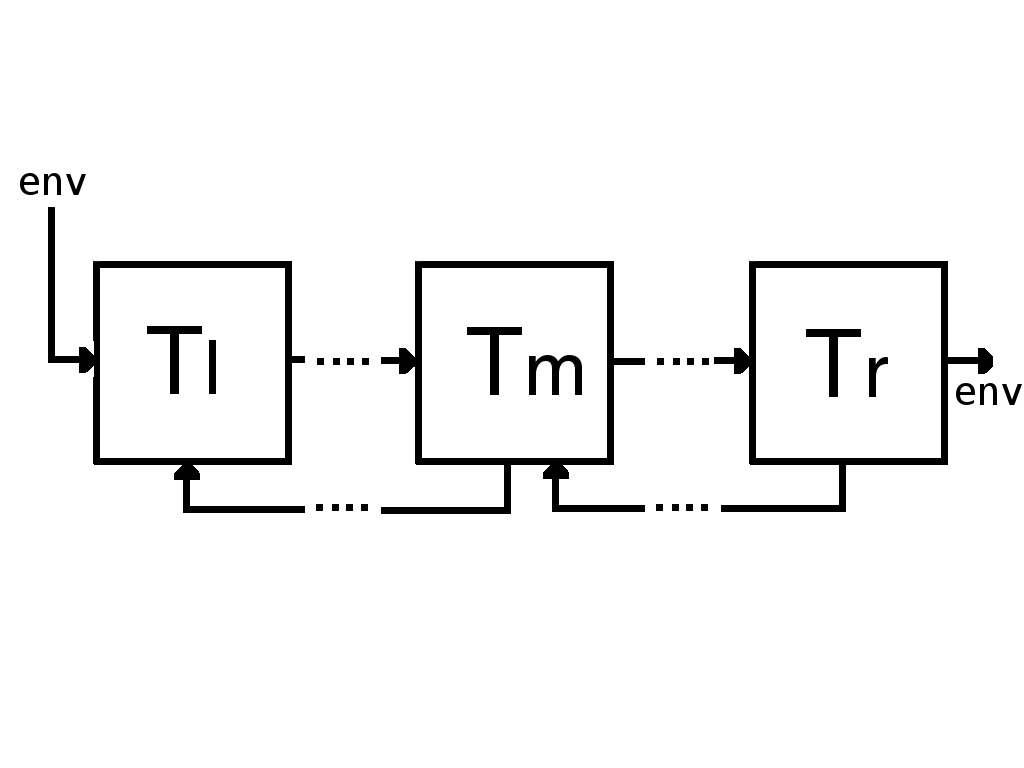
\includegraphics[width=0.9\linewidth]{TM}
\end{figure}
\end{frame}

\begin{frame} 

\begin{block}{left cell transducer:} It has two input ports, one receiving \textbf{a} from the environment and the other receiving the output of the cell on the right. It has one output to communicate with the cell to the right. $T_{l}$ starts in state $s_{init}$ (corresponding to containing $\alpha$ and being in state $q_{0}$) and on input a on input port 1 and blank on 2($(a,\epsilon)$), it mimics the instruction of M: writes $\alpha$ again, and outputs the symbol $q_{i}$ which is the state M goes into upon empty input. $T_{l}$ then goes in state $s_{\alpha}$. If $T_{l}$ receives input $q_{j}$ from the right ($(\epsilon,q_{j})$), in $s_{\alpha}$, it again does what the instruction of M requires, and outputs the new state q'. On all other inputs it outputs \textit{err} and goes in state $s_{err}$.\\
States of $S_{l}$ are $\{ s_{init},s_{\alpha},s_{err} \} $
\end{block}
\end{frame}
\begin{frame}
\begin{block}{middle cell transducer:} It has two outputs and two inputs connected to the cell on the left and the cell on the right. Input 1 and output 1 connect to the cell on the left, and input 2 and output 2 connect to the cell on the right. Input $(q, \epsilon)$ means receiving q from the left, and input $(\epsilon, q)$ means receiving q from the right. Similarly for outputs: the output $(q', \epsilon)$ corresponds to moving to the cell to the left in state q', and $(\epsilon, q')$ corresponds to moving to the cell to the right in state q'. \\
The states of $T_{m}$ are $s_{\epsilon}$ (being blank, initial state), $s_{0}$ (containing 0), $s_{1}$ (containing 1), $s_{\omega}, s_{h_{1}},...,s_{h_{t}}, s_{err}$. \\
On input q when in state $s_{c}$ the trasducer will go into state $s_{c'}$ and output q' on the left output port (if d=-1) or on the right (if d=1) output port. On all other inputs, for example input from the right when in state $s_{\epsilon}$, it goes into $s_{err}$ and outputs \textit{err}.

\end{block}
\end{frame}
\begin{frame}
\begin{block}{right cell transducer:} It has one input port from the left cell and 2 output ports, one connected to the left cell and the other connected to the environment and can be used to output \textbf{a}. This only happens when M would have gone into state $q_{n}$ (so instead of outputting $q_{n}$, $T_{r}$ outputs \textbf{a}). Otherwhise $T_{r}$ mimics M's transitions: when it is in state $s_{c}$ and receives q on the left, it goes into state $s_{c'}$ and outputs q' to the left. In all other cases, in particular when getting as input a state symbol which corresponds to moving one cell to the right to write $\omega$ in it, $T_{r}$ goes into $s_{err}$ and outputs \textit{err}. \\
The states of $T_{r}$ are $S_{r} = \{ s_{err}, s_{\omega}, s_{0}, s_{1}, s_{h_{1}},..,s_{h_{t}}, s_{err} \} .$
\end{block}

\end{frame}

\begin{frame}
\frametitle{Undecidability Proof}
Let's prove that a controller for a correctly wired composition of length k realizing T exists if and only if M halts after using k cells.\\
Suppose we have a correctly wired composition of length k. It has a free input port ($T_{l}$) and all the controller can do is to pass a to that port. On input a, $T_{l}$ starts the imitation of a Turing machine M, passing symbols corresponding to the state of M back and forth along the composition, with cell transducers changing states to represent a new symbol on the tape of M. If M halts in the kth cell of the tape, eventually $T_{r}$ gets input $q_{n}$, upon which it outputs a, and T is realized. If M does not halt, then $T_{r}$ will get an input to the right to write $\omega$ in it, and $T_{r}$ outputs err.   


\end{frame}






%PAGE26
\begin{frame}{}
  \centering \Large
  \emph{Thank you!}
\end{frame}

\end{document} 
